%% LyX 2.1.4 created this file.  For more info, see http://www.lyx.org/.
%% Do not edit unless you really know what you are doing.
\documentclass[english]{article}
\usepackage[T1]{fontenc}
\usepackage[latin9]{inputenc}
\usepackage{amsmath}
\usepackage{graphicx}

\makeatletter
%%%%%%%%%%%%%%%%%%%%%%%%%%%%%% User specified LaTeX commands.
\usepackage[margin=0.75in]{geometry} % see geometry.pdf on how to lay out the page. There's lots.
\usepackage{graphicx}
%\usepackage{cleveref}
\usepackage{amsmath}
\usepackage{multirow}
\usepackage{listings}
\usepackage{color}
\usepackage{CJK}
\definecolor{mygreen}{RGB}{28,172,0}
\definecolor{mylilas}{RGB}{170,55,241}

\usepackage[latin9]{inputenc}
\usepackage{geometry}
\geometry{verbose}


\makeatletter
\@ifundefined{date}{}{\date{}}
\makeatother

%Fancy-header package to modify header/page numbering 
\usepackage{fancyhdr}
\pagestyle{fancy}
\lhead{\textbf{ESE 101}} %name of the course
\chead{\textbf{Kangchen Bai}} %topic of the homework set
\rhead{\textbf{HW 8}} %number of the homework set
\lfoot{}
\cfoot{}
\rfoot{\thepage}


% Matlab script
\lstset{language=Matlab,%
      %basicstyle=\color{red},
  breaklines=true,%
  morekeywords={matlab2tikz},
  keywordstyle=\color{blue},%
  morekeywords=[2]{1}, keywordstyle=[2]{\color{black}},
  identifierstyle=\color{black},%}
  stringstyle=\color{mylilas},
  commentstyle=\color{mygreen},%
  showstringspaces=false,%without this there will be a symbol in the places where there is a space
  numbers=left,%
  numberstyle={\tiny \color{black}},% size of the numbers
  numbersep=9pt, % this defines how far the numbers are from the text
  emph=[1]{for,end,break},emphstyle=[1]\color{red}, %some words to emphasise
                                                      %emph=[2]{word1,word2}, emphstyle=[2]{style},    
}

\makeatother

\usepackage{babel}
\begin{document}

\subsection*{(a)}

We find the following relation between $D$ ,$(x-\xi)$ and $\theta$:

$cos\theta=\frac{D}{(D^{2}+(x-\xi)^{2})^{1/2}}$ $sin\theta=\frac{(x-\xi)}{(D^{2}+(x-\xi)^{2})^{1/2}}$

The directional vector: $\hat{r}=\begin{bmatrix}cos\theta\\
sin\theta
\end{bmatrix}$

$\Delta F=\begin{bmatrix}M\Delta g_{z}\\
M\Delta g_{x}
\end{bmatrix}=\frac{GM\Delta m}{r^{2}}\hat{r}=\frac{GM\Delta m}{D^{2}+(x-\xi)^{2}}\begin{bmatrix}cos\theta\\
sin\theta
\end{bmatrix}=\begin{bmatrix}\frac{GM\Delta mD}{(D^{2}+(x-\xi)^{2})^{3/2}}\\
\frac{GM\Delta m(x-\xi)}{(D^{2}+(x-\xi)^{2})^{3/2}}
\end{bmatrix}$

so $\Delta g_{z}=\frac{G\Delta mD}{(D^{2}+(x-\xi)^{2})^{3/2}}$


\subsection*{(b)}

Because the anomalies are at 0.1 meter intervals from 0 to 10, we
consider the k anomaly:

$\xi=0.1(k-1)$

$g(x,\Delta m_{k})=\frac{GD\Delta m_{k}}{[D^{2}+(x-0.1(k-1))^{2}]^{3/2}}$

so the total contribution of all anomalies can be calculated as 

$g(x,m)=\underset{k=1}{\overset{101}{\sum}}\frac{GD\Delta m_{k}}{[D^{2}+(x-0.1(k-1))^{2}]^{3/2}}$
where $m=[\Delta m_{1}\Delta m_{2}...\Delta m_{101}]'$


\subsection*{(c)}

Linear. Because the model predication is a linear function of $m$:

\begin{eqnarray*}
\boldsymbol{d_{i}} & = & \boldsymbol{G_{i,:}}\mbox{\ensuremath{\boldsymbol{m}}}
\end{eqnarray*}


where

\begin{eqnarray*}
\boldsymbol{G_{ij}} & = & \frac{GD}{\left[D^{2}+(x_{i}-0.1\cdot(j-1))^{2}\right]^{3/2}}
\end{eqnarray*}



\subsection*{(d)}

\begin{figure}
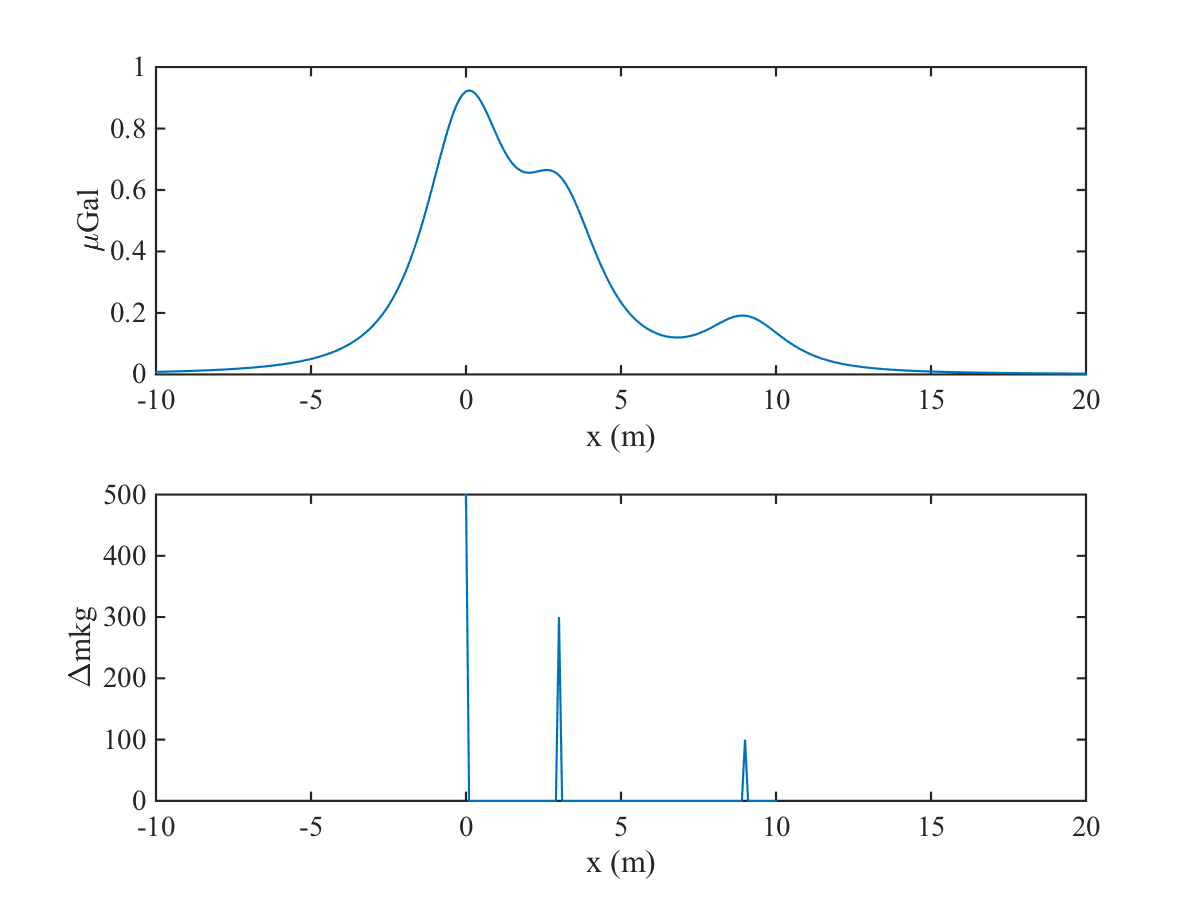
\includegraphics[width=15cm]{figure/d}\caption{}


\end{figure}



\subsection*{(e)}

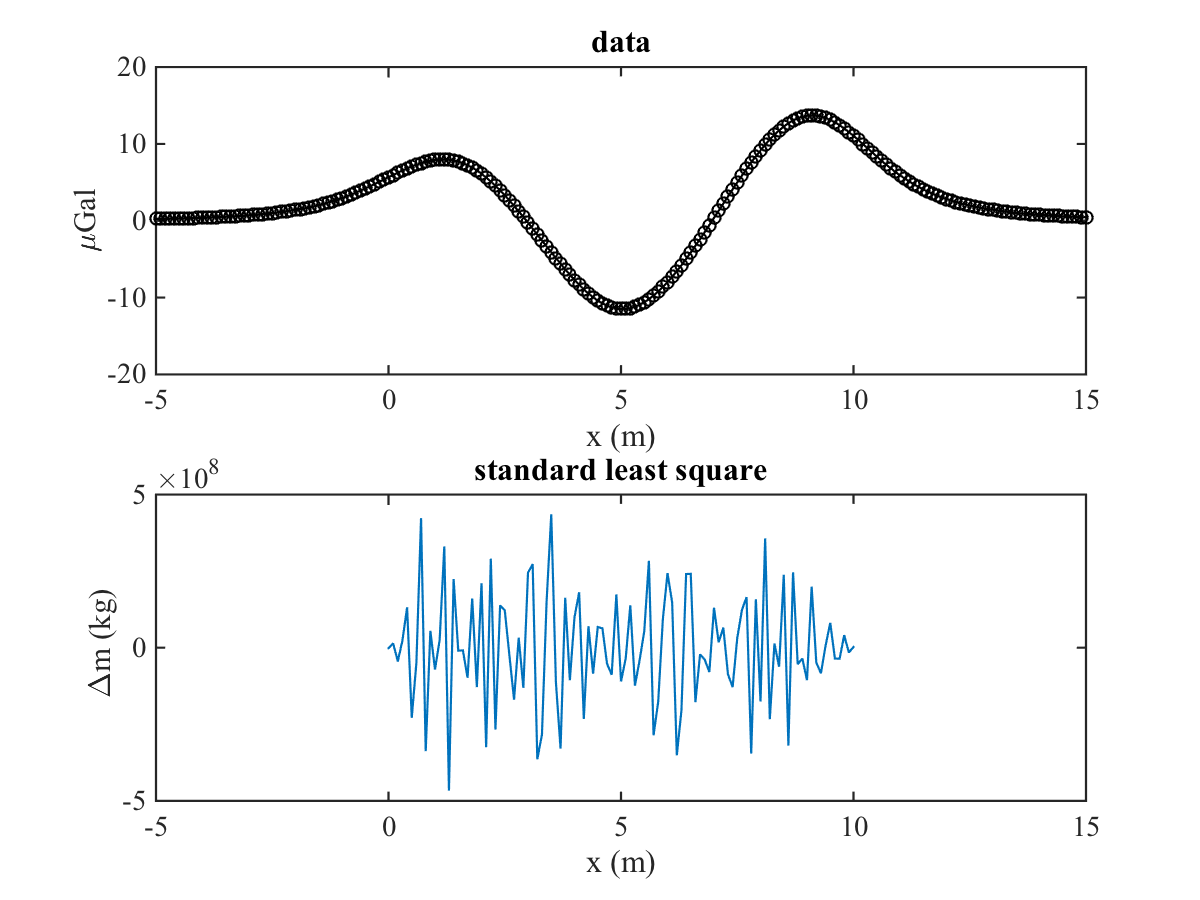
\includegraphics[width=15cm]{figure/e_result}

We see that the inversion result is messy. To understand it, we calculate
the singular values, and plot them in logarithm.

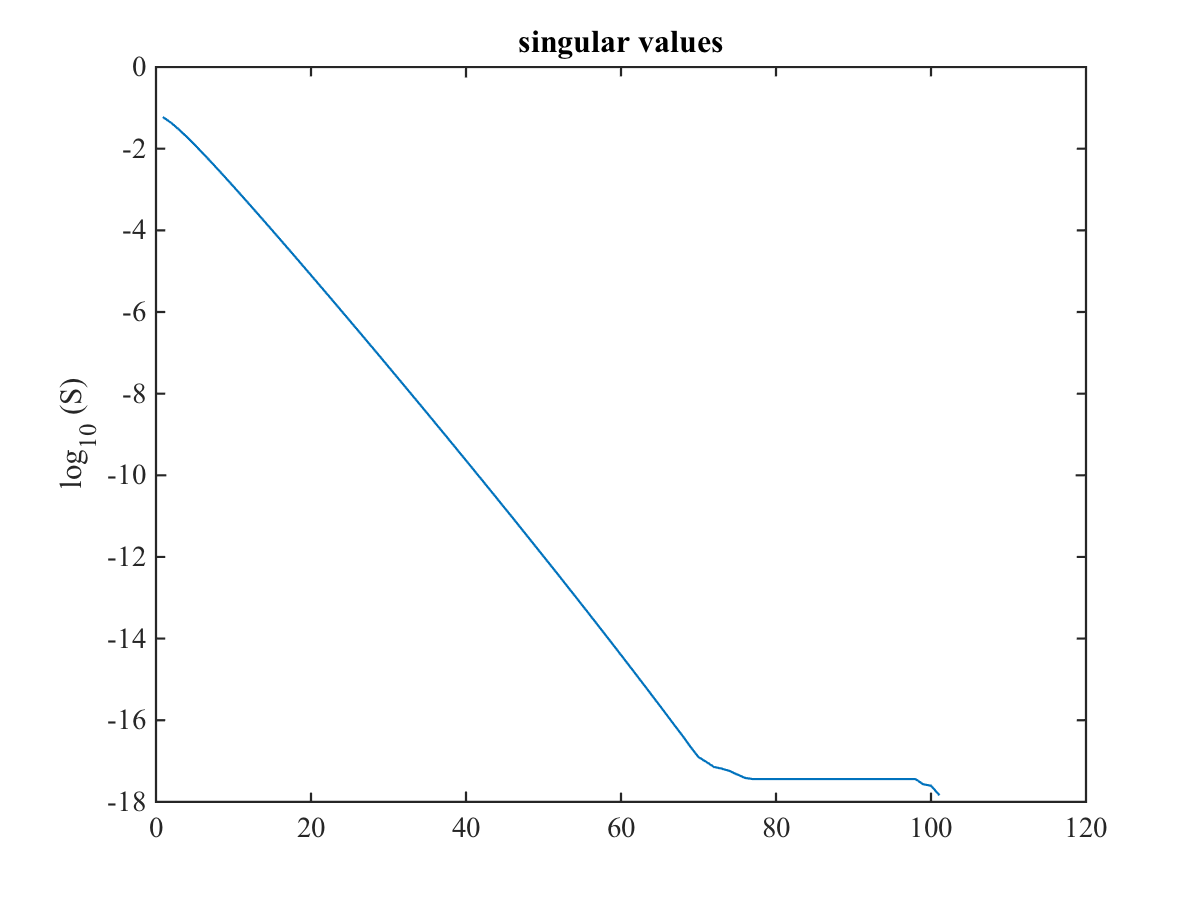
\includegraphics[width=15cm]{figure/e_snv}

We see that, ..


\subsection*{(f)}

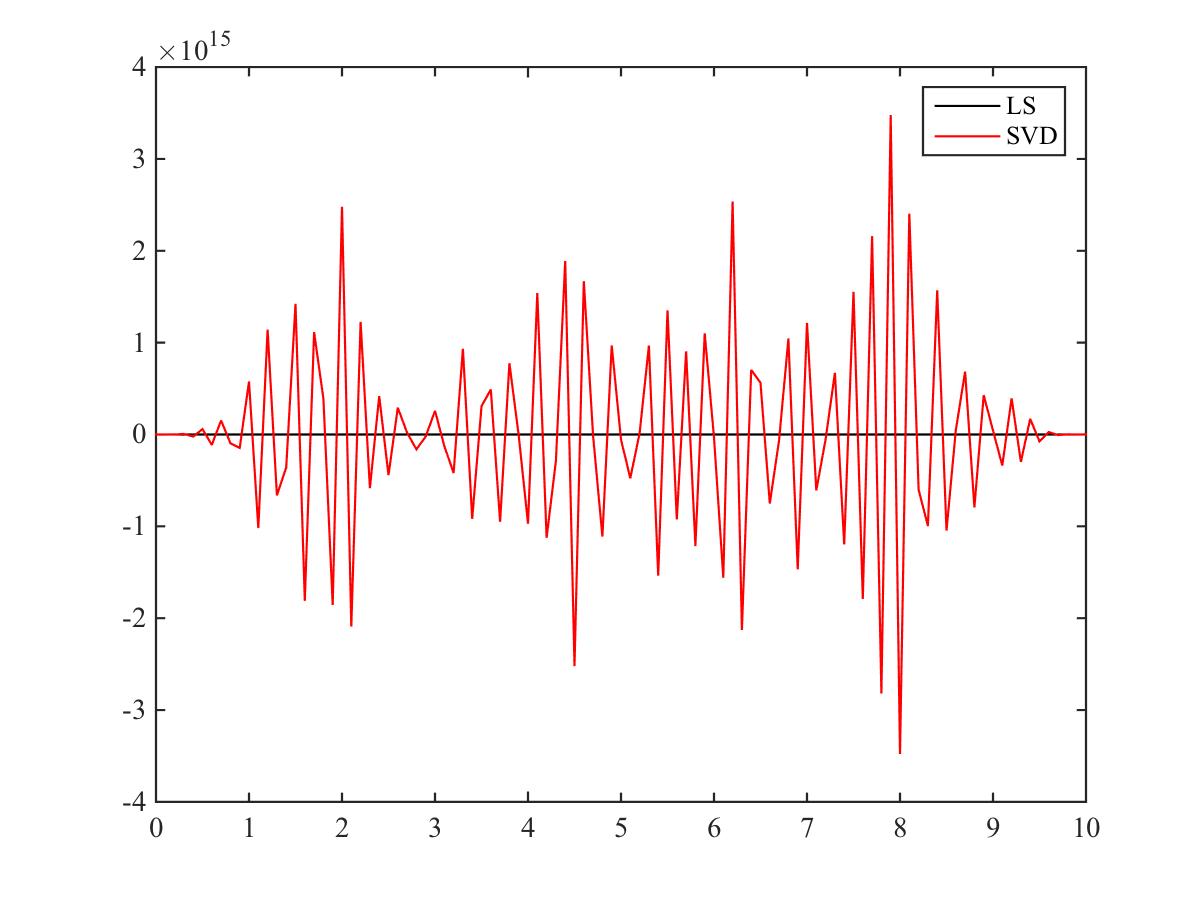
\includegraphics[width=15cm]{figure/f}

(g)

\begin{figure}


\caption{}


\end{figure}


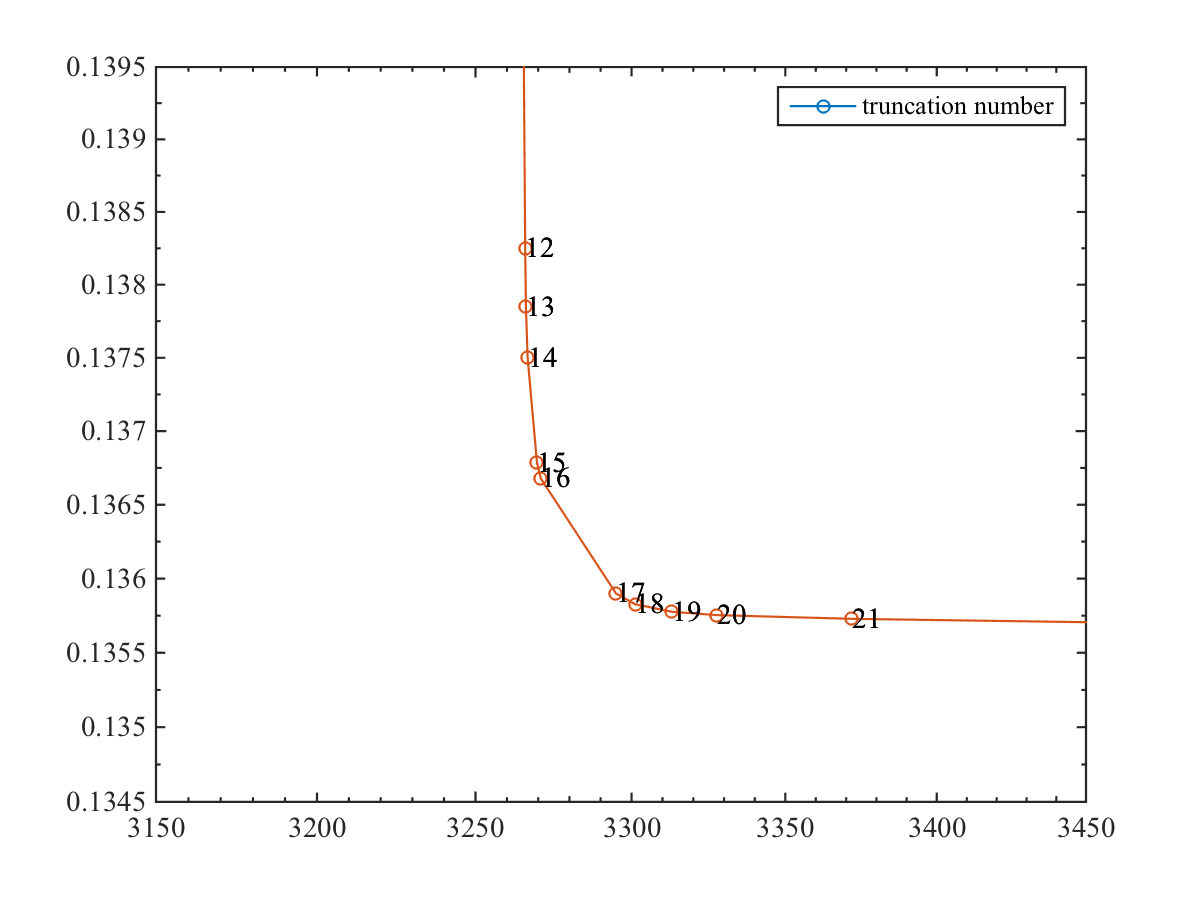
\includegraphics[width=15cm]{figure/g_trunc}

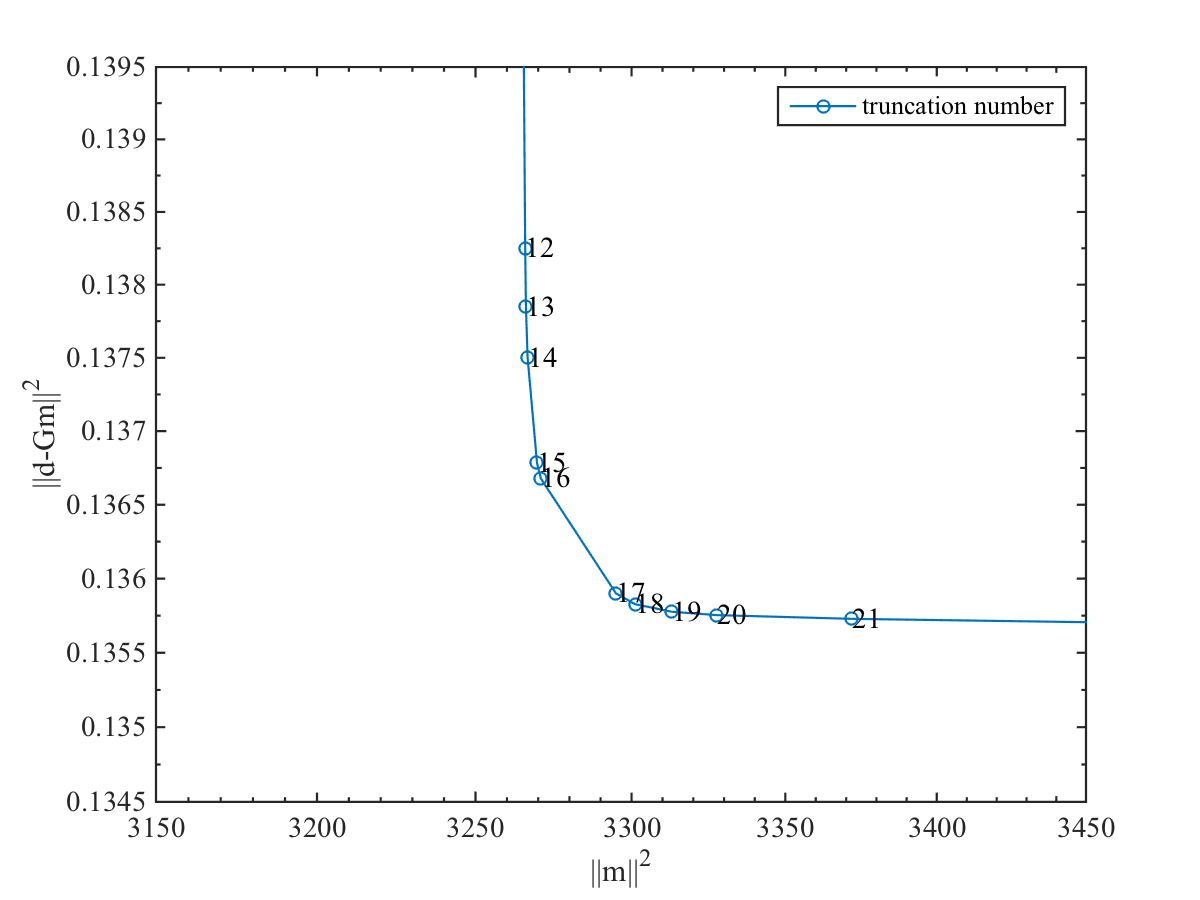
\includegraphics[width=15cm]{figure/g_trunc_zoomin}


\end{document}
